
%(BEGIN_QUESTION)
% Copyright 2010, Tony R. Kuphaldt, released under the Creative Commons Attribution License (v 1.0)
% This means you may do almost anything with this work of mine, so long as you give me proper credit

Bestem effekten av hver feil - vurdert én om gangen - på driften av denne ikke-dispersive infrarøde (NDIR) analysatoren:

$$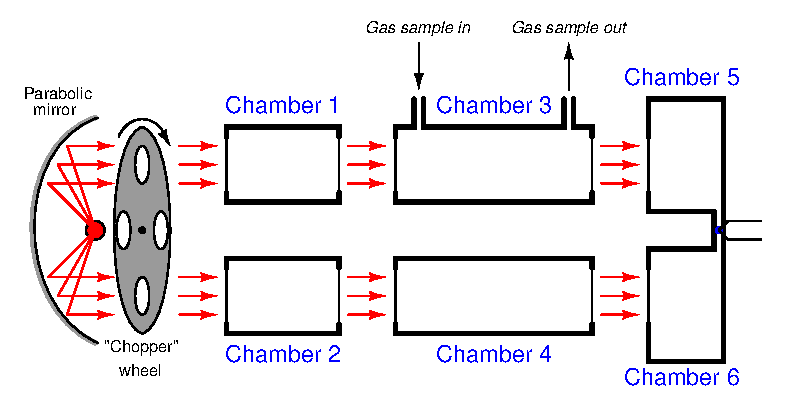
\includegraphics[width=15.5cm]{i00758x01.eps}$$

\begin{itemize}
\item{} Hakkehjulet slutter å rotere
\vskip 10pt
\item{} Det oppstår lekkasje i kammer 2
\vskip 10pt
\item{} Det oppstår lekkasje i kammer 4
\vskip 10pt
\item{} Det parabolske speilet sprekker
\end{itemize}

\underbar{file i00758}
%(END_QUESTION)





%(BEGIN_ANSWER)

\begin{itemize}
\item{} Hakkehjulet slutter å rotere: {\it analysatorens utgang vil gå til null for alle gasskonsentrasjoner.}
\vskip 10pt
\item{} Det oppstår lekkasje i kammer 2: {\it en «nullpunktsforskyvning» vil oppstå.}
\vskip 10pt
\item{} Det oppstår lekkasje i kammer 4: {\it det kan hende det ikke blir noen effekt, med mindre omgivelsesluften inneholder en betydelig konsentrasjon av en interfererende gass.}
\vskip 10pt
\item{} Det parabolske speilet sprekker: {\it nullpunktsforskyvning, avhengig av hvor sprekken sitter og hvor alvorlig den er.}
\end{itemize}


%(END_ANSWER)





%(BEGIN_NOTES)


%INDEX% Måling, analytisk: ikke-dispersiv optisk

%(END_NOTES)

